\section{Topología en el espacio euclídeo}
\begin{definición}[Longitud o Norma euclídea]
    Se denomina \textbf{longitud} o \textbf{norma euclídea} de un vector $\vec{x} = (x_1, x_2, \ldots, x_n) \in \mathbb{R}^n$ al númeor real mayor o igual que cero definido por $$\|\vec{x}\| = \sqrt{x_1^2 + x_2^2 + \ldots + x_n^2}.$$
\end{definición}

\begin{definición}[Distancia euclídea]
    Se llama \textbf{distancia euclídea} entre dos vectores $\vec{x} = (x_1, x_2, \ldots, x_n)$ y $\vec{y} = (y_1, y_2, \ldots, y_n)$ al número real mayor o igual que 0 definido por:
    \[
        d(\vec{x}, \vec{y}) = \|\vec{x} - \vec{y}\| = \left( \sum_{i = 1}^{n} (x_i - y_i)^2 \right)^{\frac{1}{2}}
    \]
\end{definición}

\begin{definición}[Producto escalar euclídeo]
    Se llama \textbf{producto escalar euclídeo} entre dos vectores $\vec{x} = (x_1, x_2, \ldots, x_n)$ y $\vec{y} = (y_1, y_2, \ldots, y_n)$ al número real, no necesariamente positivo, definido por:
    $$\langle \vec{x}, \vec{y} \rangle = x_1 y_1 + x_2 y_2 + \ldots + x_n y_n = \sum_{i = 1}^{n} x_i y_i.$$
\end{definición}


\begin{teorema}
    \begin{enumerate}
        \item $\langle \vec{x}, \vec{y} \rangle \geq 0 \quad \forall \vec{x}, \vec{y} \in \mathbb{R}^n$.
        \item $\langle \vec{x}, \vec{y} \rangle = 0 \Leftrightarrow \vec{x} = \vec{0}$ o $\vec{y} = \vec{0}$.
        \item $\forall \vec{x}, \vec{y}, \vec{z} \in \mathbb{R}^n \text{ se cumple que } \langle \vec{x} + \vec{y}, \vec{z} \rangle = \langle \vec{x}, \vec{z} \rangle + \langle \vec{y}, \vec{z} \rangle$.
        \item $\langle \alpha \vec{x}, \vec{y} \rangle = \alpha \langle \vec{x}, \vec{y} \rangle$ para todo $\alpha \in \mathbb{R}$.
        \item $\langle \vec{x}, \vec{y} \rangle = \langle \vec{y}, \vec{x} \rangle$.
    \end{enumerate}
\end{teorema}

\begin{teorema}
    Para cualesquiera $x, \in \mathbb{R}^2$ se verifica que $\langle x, y\rangle = \|\vec{x}\| \|\vec{y}\| \cos(\theta)$, donde $\theta$ es el ángulo entre los vectores $\vec{x}$ y $\vec{y}$.
\end{teorema}
\begin{proof}
    Dados dos vectores \( x \) e \( y \) de \( \mathbb{R}^2 \), que supondremos distintos de 0 (pues si uno de ellos es 0 el resultado es inmediato), consideremos el triángulo de vértices \( 0 \), \( x \), \( y \):
    
    
    \begin{center}
    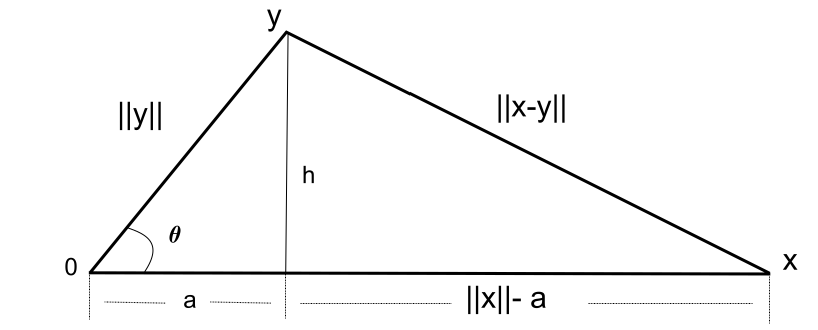
\includegraphics[width=0.5\textwidth]{Graphics/triangulo.png} % Reemplaza con tu gráfico si quieres incluir uno.
    \end{center}
    Utilizando trigonometría elemental, tenemos que:
    \[
    \cos \theta = \frac{a}{\|y\|}
    \]

    Además, usando el teorema de Pitágoras, tenemos que:
    $$ \|y\|^2 = a^2 + h^2 \implies \|y\|^2 - a^2 = h^2 = \|x - y\|^2 - (\|x\| - a)^2$$

    Con lo que:
    \[
    \|x - y\|^2 = \|y\|^2 - a^2 + \|x\|^2 - 2a\|x\| + a^2 = \|y\|^2 + \|x\|^2 - 2a\|x\|
    \]

    Usando que \( a = \|y\|\cos\theta \), obtenemos:
    \[
    \|x - y\|^2 = \|x\|^2 + \|y\|^2 - 2\|x\|\|y\|\cos\theta
    \]

    Si ahora usamos las propiedades del producto interior, obtenemos que:
    \[
    \|x - y\|^2 = \langle x - y, x - y \rangle = \|x\|^2 - 2\langle x, y \rangle + \|y\|^2
    \]

    De donde se deduce, teniendo en cuenta el valor previamente obtenido de \( \|x - y\|^2 \), que:
    \[
    \langle x, y \rangle = \|x\| \|y\| \cos\theta
    \]
\end{proof}

\begin{definición}[Vectores ortogonales]
    Se dice que dos vectores \( \vec{x} \) y \( \vec{y} \) son \textbf{ortogonales} si $\langle \vec{x}, \vec{y} \rangle = 0$.
\end{definición}

\begin{proposición}[Propiedades de la norma euclídea]
    \begin{enumerate}
        \item $\|\vec{x}\| \geq 0 \quad \forall \vec{x} \in \mathbb{R}^n$.
        \item $\|\vec{x}\| = 0 \Leftrightarrow \vec{x} = \vec{0}$.
        \item $\|\alpha \vec{x}\| = |\alpha| \|\vec{x}\|$ para todo $\alpha \in \mathbb{R}$.
        \item $\|\vec{x} + \vec{y}\| \leq \|\vec{x}\| + \|\vec{y}\| \quad \forall \vec{x}, \vec{y} \in \mathbb{R}^n$ (desigualdad triangular).
    \end{enumerate}
\end{proposición}

\begin{teorema}[Desigualdad de Cauchy-Schwarz]
    Sea \( \vec{x}, \vec{y} \in \mathbb{R}^n \). Entonces se cumple que:
    \[
        |\langle \vec{x}, \vec{y} \rangle| \leq \|\vec{x}\| \|\vec{y}\|
    \]

    Equivalentemente 
    $$\left\|\sum_{i=1}^{n} x_i y_i\right\| \leq \sqrt{\sum_{i=1}^{n} x_i^2} \sqrt{\sum_{i=1}^{n} y_i^2}$$
    
\end{teorema}

\begin{proof}
    Fijemos $\vec{x}$ y $\vec{y} \in \mathbb{R}^n$. Para cada $\alpha \in \mathbb{R}$ se tiene que 
    $$\langle \alpha \vec{x} + \vec{y}, \alpha \vec{x} + \vec{y} \rangle  = \alpha^2 \langle , \rangle + 2\alpha \langle x, y\rangle + \langle y, y \rangle \geq 0$$
    Si tomamos $A = \langle \vec{x}, \vec{x} \rangle$, $B = 2\langle \vec{x}, \vec{y} \rangle$ y $C = \langle \vec{y}, \vec{y} \rangle$, tenemos que: 
    $$A\alpha^2 + B\alpha + C \geq 0 \quad \forall \alpha \in \mathbb{R}$$
    Entoncespodemos distinguir dos casos:
    \begin{enumerate}
        \item Si \( A = 0 \), entonces \( \vec{x} = \vec{0} \) y la desigualdad es trivial.
        \item Si \( A > 0 \), entonces la desigualdad anterior es una ecuación cuadrática en \( \alpha \), y por las propiedades del producto escalar es necasrio que su discriminantes sea no positivo, pues de lo contrario tendría dos raíces reales distintias y entonces la ecuacion tomaría algún valor negativo 
        $$\implies D = B^2 - 4AC \leq 0 \iff B^2 \leq 4AC \iff 4\langle \vec{x}, \vec{y} \rangle^2 \leq 4\langle \vec{x}, \vec{x} \rangle \langle \vec{y}, \vec{y} \rangle = 4\|x\|^2 \|y\|^2$$
    \end{enumerate}

\end{proof}

\begin{proposición}[Propiedades de la distancia euclídea]
    \begin{enumerate}
        \item $d(\vec{x}, \vec{y}) \geq 0 \quad \forall \vec{x}, \vec{y} \in \mathbb{R}^n$.
        \item $d(\vec{x}, \vec{y}) = 0 \Leftrightarrow \vec{x} = \vec{y}$.
        \item $d(\vec{x}, \vec{y}) = d(\vec{y}, \vec{x})$.
        \item $d(\vec{x}, \vec{z}) \leq d(\vec{x}, \vec{y}) + d(\vec{y}, \vec{z})$ (desigualdad triangular).
    \end{enumerate}
\end{proposición}

\begin{definición}[Métrica]
    Se llama \textbf{métrica} sobre un conjunto arbitrario $M$ a cualquier aplicación $d: M \times M \to \mathbb{R}$ que cumple las siguientes propiedades:
    \begin{enumerate}
        \item $d(x, y) \geq 0 \quad \forall x, y \in M$.
        \item $d(x, y) = 0 \Leftrightarrow x = y$.
        \item $d(x, y) = d(y, x)$.
        \item $d(x, z) \leq d(x, y) + d(y, z)$ (desigualdad triangular).
    \end{enumerate}
\end{definición}

\begin{definición}[Espacio métrico]
    Se llama \textbf{espacio métrico} a un par $(M, d)$ donde $M$ es un conjunto no vacío y $d$ es una métrica sobre $M$.
\end{definición}

\ejemplo{
    Vemos algunos ejemploes de métricas: 
    \begin{enumerate}
        \item La métrica euclídea en $\mathbb{R}^n$ 
        \item $d_1(x, y) = \sum_{i = 1}^{n} |x_i - y_i|$ 
        \item $d_\infty(x, y) = \max_{i = 1, \ldots, n} |x_i - y_i|$
        \item $d(f, g) = \int_{a}^{b} |f(x) - g(x)| dx$ para funciones $f, g: [a, b] \to \mathbb{R}$.
        \item $d_{\infty}(f, g) = \max_{x \in [a, b]} |f(x) - g(x)|$ para funciones $f, g: [a, b] \to \mathbb{R}$.
        \item $d(x, y) = \begin{cases}
            0 & \text{si } x = y \\
            1 & \text{si } x \neq y
        \end{cases}$, que se conoce como la \textbf{métrica discreta}.
    \end{enumerate}
}

\begin{definición}[Diámetro]
    Se llama \textbf{diámetro} de un subconjunto $S$ de un espacio métrico $(M, d)$ a
    $$diam(S) = \sup\{d(x, y) \mid x, y \in S\}$$
    si el conjunto de números reales $\{d(x,y) : x,y \in S\}$ es acotado superiormente y se define $diam(S) = +\infty$ en caso contrario. Cuando el diámetro es infinito se dice que el conjunto no es \textbf{acotado}.
\end{definición}

\begin{definición}[Norma]
    Sea $V$ un espacio vectorial sobre $\mathbb{R}$. Se llama \textbf{norma} en $V$ a toda aplicación $\|\cdot\|: V \to \mathbb{R}$ que cumple las siguientes propiedades:
    \begin{enumerate}
        \item $\|\vec{x}\| \geq 0 \quad \forall \vec{x} \in V$.
        \item $\|\vec{x}\| = 0 \Leftrightarrow \vec{x} = \vec{0}$.
        \item $\|\alpha \vec{x}\| = |\alpha| \|\vec{x}\|$ para todo $\alpha \in \mathbb{R}$.
        \item $\|\vec{x} + \vec{y}\| \leq \|\vec{x}\| + \|\vec{y}\|$ (desigualdad triangular).
    \end{enumerate}
\end{definición}

\ejemplo{
    \begin{enumerate}
        \item $\|\vec{x}\| = |x|$
        \item $\|\vec{x}\|_2 = \left(\sum_{j = 1}^{n} x_j^2\right)^{\frac{1}{2}}$ (norma euclídea).
        \item $\|\vec{x}\|_1 = \sum_{j = 1}^{n} |x_j|$ (norma $l^1$).
        \item $\|\vec{x}\|_\infty = \max_{j = 1, \ldots, n} |x_j|$ (norma $l^\infty$).
        \item $\|f\|_{\infty} = \max_{x \in [a, b]} |f(x)|$ para funciones $f: [a, b] \to \mathbb{R}$.
    \end{enumerate}
}

\begin{definición}[Producto escalar o interior]
    Llamaremos producto escalar o producto interior en $V$ a toda aplicación $\langle \cdot, \cdot \rangle: V \times V \to \mathbb{R}$ que cumple las siguientes propiedades:
    \begin{enumerate}
        \item $\langle \vec{x}, \vec{y} \rangle \geq 0 \quad \forall \vec{x}, \vec{y} \in V$.
        \item $\langle \vec{x}, \vec{x} \rangle = 0 \Leftrightarrow \vec{x} = \vec{0}$.
        \item $\langle \vec{x}, \vec{y} \rangle = \langle \vec{y}, \vec{x} \rangle$.
        \item $\langle \alpha \vec{x}, \vec{y} \rangle = \alpha \langle \vec{x}, \vec{y} \rangle$ para todo $\alpha \in \mathbb{R}$.
        \item $\langle \vec{x} + \vec{y}, \vec{z} \rangle = \langle \vec{x}, \vec{z} \rangle + \langle \vec{y}, \vec{z} \rangle$ para todo $\vec{x}, \vec{y}, \vec{z} \in V$.
    \end{enumerate}
\end{definición}

\begin{definición}[Igualdad del paralelogramo]
    Sea una norma $\|\cdot\|$ en un espacio vectorial $V$. Se dice que la norma cumple la \textbf{igualdad del paralelogramo} si la norma procede de un producto escalar
    $$\|\vec{x} + \vec{y}\|^2 + \|\vec{x} - \vec{y}\|^2 = 2\|\vec{x}\|^2 + 2\|\vec{y}\|^2$$
\end{definición}
\begin{proof}
    $$\|\vec{x} + \vec{y}\|^2 + \|\vec{x} - \vec{y}\|^2 = \langle \vec{x} + \vec{y}, \vec{x} + \vec{y} \rangle + \langle \vec{x} - \vec{y}, \vec{x} - \vec{y} \rangle = $$
    $$ = \|\vec{x}\|^2 + \langle \vec{x}, \vec{y} \rangle + \langle \vec{y}, \vec{x} \rangle + \|\vec{y}\|^2 + \|\vec{x}\|^2 - \langle \vec{x}, \vec{y} \rangle - \langle \vec{y}, \vec{x} \rangle + \|\vec{y}\|^2 = 2\|\vec{x}\|^2 + 2\|\vec{y}\|^2$$
\end{proof}

\begin{definición}[Bola abierta]
    Dados $x_0 \in \mathbb{R}^n$ y un número real $r > 0$, llamamos \textbf{bola abierta} de centro $x_0$ y radio $r$ al conjunto
    $$B(x_0, r) = \{x \in \mathbb{R}^n \mid d(x, x_0) < r\}$$
    donde $d$ es la métrica que se está considerando en $\mathbb{R}^n$.
\end{definición}

\begin{definición}[Conjunto abierto]
    Se dice que un conjunto $A \subset \mathbb{R}^n$ es \textbf{abierto} si para todo punto $x_0 \in A$ existe un número real $r > 0$ tal que $B(x_0, r) \subset A$.
\end{definición}

\begin{proposición}[Propiedades de los conjuntos abiertos]
    \begin{enumerate}
        \item El conjunto vacío y el espacio euclídeo $\mathbb{R}^n$ son abiertos.
        \item La unión de abiertos es un abierto
        \item La interseccion finita de abiertos es un abierto.
    \end{enumerate}
\end{proposición}

\begin{definición}[Punto abierto]
    Se dice que un punto $x \in S \subset \mathbb{R}^n$ es un \textbf{punto abierto} de $S$ si existe una bola abierta $B(x, r)$ tal que $B(x, r) \subset S$. Denotamos por $S^\circ$ al conjunto de los puntos abiertos de $S$.
\end{definición}

\begin{observación}
    $S^\circ$ puede ser vacío, por ejemplo si $S$ es un subconjunto con un solo punto
\end{observación}

\begin{proposición}[Propiedades de los puntos abiertos]
    \begin{enumerate}
        \item $S^\circ$ es el mayor abierto contenido en $S$
        \item $S^\circ$ es la unión de todos los abiertos contenidos en $S$.
        \item $S$ es abierto si y solo si $S = S^\circ$.
    \end{enumerate}
\end{proposición}
\begin{proof}
    \begin{enumerate}
        \item $S^\circ$ es abierto, pues dado $x \in S^\circ$, existe $r > 0$ tal que $B(x, r) \subset S$. Entonces sucede que $B(x, r) \subset S^\circ$, pues al ser $B(x, r)$ un abierto, entonces $B(x, r) = [B(x, r)]^{\circ} \subset S^\circ$. Por otra parte, si $A$ es un abierto de $\mathbb{R}^n$ contenido en $S$, entonces para todo punto de A hay una bola centrada en él contenida en $A$ y por lo tanto en $S$, lueg todos los puntos de $A$ están en $S^\circ$
        \item Es claro que el mayor abierto contenido en $S$ es la unión de todos los abiertos contenidos en $S$
        \item Si $S$ es abierto, entonces él es el mayor abierto contenido en $S$, luego $S = S^\circ$. Por otra parte, si $S = S^\circ$, entonces $S$ es abierto, pues para todo punto $x \in S$, existe una bola abierta $B(x, r)$ tal que $B(x, r) \subset S$, luego $S$ es abierto.	
    \end{enumerate}
\end{proof}

\begin{definición}[Bola cerrada]
    Dados $x_0 \in \mathbb{R}^n$ y un número real $r > 0$, llamamos \textbf{bola cerrada} de centro $x_0$ y radio $r$ al conjunto
    $$\overline{B}(x_0, r) = \{x \in \mathbb{R}^n \mid d(x, x_0) \leq r\}$$
\end{definición}
\begin{proposición}
    Sea $x_0 \in \mathbb{R}^n$ y $r > 0$. Entonces se cumple que: 
    $$[\overline{B}(x_0, r)]^\circ = B(x_0, r)$$
\end{proposición}
\begin{proof}
    ``$\subset$''

    $$ \text{Sea } x \in [\overline{B}(x_0, r)]^\circ \implies \exists r_x > 0 : B(x, r_x) \subset \overline{B}(x_0, r) \text{ tal que } \|x - x_0\| = r$$
    $$\text{Sea } y = x + \frac{x - x_0}{\|x - x_0\|} \cdot \frac{1}{2} r_x \implies \|y - x\| = \frac{1}{2} r_x < r_x \implies y \in B(x, r_x)$$ 
    No obstante, 
    $$\|y- x_0\| = \|x- x_0\|\left(1 + \frac{1}{\|x - x_0\|}\frac{1}{2}r_x\right) > \|x - x_0| = r$$ 
    Por tanto llegamos a que ningún punto de la frontera de la bola cerrada puede estar en su interior.
    ``$\supset$''
    \begin{quote}
    Esta inclusión es inmediata pues $B(x_0, r) \subset \overline{B}(x_0, r)$ y al ser $B(x_0, r) = \left[B(x_0, r)\right]^{\circ}$ resulta que $B(x_0, r) \subset \left[\overline{B}(x_0, r)\right]^{\circ}$.
    \end{quote}
\end{proof}

\begin{definición}[Conjunto cerrado]
    Se dice que un subcnjunto $C \subset \mathbb{R}^n$ es \textbf{cerrado} si su complementario (respecto a $\mathbb{R}^n$) es abierto. 
\end{definición}
\begin{proposición}[Propiedades de los conjuntos cerrados]
    \begin{enumerate}
        \item El conjunto vacío y el espacio euclídeo $\mathbb{R}^n$ son cerrados.
        \item La intersección de cerrados es un cerrado.
        \item La unión finita de cerrados es un cerrado.
    \end{enumerate}
\end{proposición}
\begin{definición}[Punto de acumulación]
    Se dice que un punto $x \in \mathbb{R}^n$ es un \textbf{punto de acumulación} de un subconjunto $S \subset \mathbb{R}^n$ si toda bola abierta centrada en $x$ contiene algún punto de S distinto de $x$. Equivalentemente, 
    $$x \text{ es un punto de acumulación de } S \Leftrightarrow \forall r > 0, B(x, r) \cap (S \setminus \{x\}) \neq \emptyset$$
    Al conjunto de puntos de acumulación de un conjunto se le suele denominar $S \prime$ 
\end{definición}
\ejemplo{
    \begin{enumerate}
        \item Todo punto del intervalo $[0,1]$ es un punto de acumulación de $(0,1)$.
        \item El punto $0$ es un punto de acumulación de $S = \{1/n \mid n \in \mathbb{N}\}$
        \item $S = \mathbb{Q} \cap [0, 1] \implies S' = [0, 1]$.
    \end{enumerate}
}

\begin{teorema}
    $S$ es cerrado si y solo si $S' \subset S$.
\end{teorema}
\begin{proof}
    ``$\Rightarrow$``
    Supongamos que $S$ es cerrado. Entonces sea $x \in S' : x \notin S \implies $ cualquier bola de centro en  $x$ contiene puntos de $S \implies \mathbb{R}^n \setminus S$ no es abierto, luego llegamos a contradicción y que $x \in S$.

    ``$\Leftarrow$``
    Dado $x \in \mathbb{R}^n \setminus S \implies \exists r > 0 : B(x, r) \subset \mathbb{R}^n \setminus S$ (pues $x$ no es punto de acumulación de $S$). Por tanto, $B(x, r) \subset \mathbb{R}^n \setminus S$, luego $\mathbb{R}^n \setminus S$ es abierto y por tanto $S$ es cerrado.
\end{proof}
\begin{definición}[Punto adherente]
    Se dice que un punto $x \in \mathbb{R}^n$ es un \textbf{punto adherente} de un subconjunto $S \subset \mathbb{R}^n$ si toda bola abierta centrada en $x$ contiene algún punto de S. Equivalentemente,
    $$x \text{ es un punto adherente de } S \Leftrightarrow \forall r > 0, B(x, r) \cap S \neq \emptyset$$
\end{definición}
\begin{definición}[Adherencia o clausura]
    Se llama \textbf{adherencia} o \textbf{clausura} de un conjunto $S \subset \mathbb{R}^n$ al conjunto de sus puntos adherentes, denotado por $\overline{S}$.
\end{definición}

\begin{proposición}[Propiedades de la adherencia]
    \begin{enumerate}
        \item $\overline{S}$ es cerrado y es el menor cerrado que contiene a $S$ ($S \subset \overline{S}$)
        \item $\overline{S}$ es la intersección de todos los cerrados que contienen a $S$.
        \item $S$ es cerrado si y solo si $S = \overline{S}$.
    \end{enumerate}
\end{proposición}
\begin{proof}
    \begin{enumerate}
        \item Sea $x \in \mathbb{R}^n \setminus \overline{S} \implies \exists r > 0 : B(x, r) \cap S = \emptyset \implies \forall y \in B(x, r) : B(y, r - d(y,x)) \cap S = \emptyset \implies y \notin \overline{S} \implies B(x,r) \subset \mathbb{R}^n \setminus \overline{S}$. \newline
        Por otro lado, si $C$ es un cerrado que contiene a $S$, entonces $C$ debe contener a $\overline{S}$, pues C cntiene a S y a $S'$ debido a que $S' \subset C' \subset C$ por ser $C$ cerrado. 
        \item Es claro que el menor cerrado que contiene a un conjunto es la intersección de todos los cerrados que lo contienen. Además, la intersección finita de cerrados es cerrada. 
        \item Si $S$ es cerrado es claro que él mismo es el menor cerrado que lo contiene, luego $S = \overline{S}$. Recíprocamente, por lo visto en el primer apartado, si $\overline{S}$ es cerrado, entonces si $S = \overline{S}$, entonces $S$ es cerrado.
    \end{enumerate}
\end{proof}

\begin{definición}[Distancia]
    Dados un conjunto $S \subset \mathbb{R}^n$ y un punto $x \in \mathbb{R}^n$, se define la \textbf{distancia} de $x$ a $S$ como
    $$d(x, S) = \inf\{d(x, y) : y \in S\}$$
\end{definición}

\begin{teorema}
    Un punto $x \in \mathbb{R}^n$ es un punto adherente de un conjunto $S \subset \mathbb{R}^n$ si y solo si $d(x, S) = 0$.
\end{teorema}
\begin{proof}
    ``$\rightarrow$``
    $x \in \overline{S} \implies \forall r > 0, \exists y \in S : d(x, y) < r \implies \inf\{d(x, y) : y \in S\} = 0$. Obsérvese que como $x \in S$ este ínfimo se alcanza y es mínimo. 

    ``$\leftarrow$``
    El $\inf\{d(x, y) : y \in S\} = 0$ implica que $\forall \epsilon > 0, \exists y \in S : d(x, y) < \epsilon$. Entonces$B(x, \epsilon) \cap S \neq \emptyset$, luego $x$ es un punto adherente de $S$.
\end{proof}
\begin{definición}[Punto frontera]
    Se llama \textbf{punto frontera} de un conjunto $S \subset \mathbb{R}^n$ a todo punto $x \in \mathbb{R}^n$ tal que $\forall r > 0$, se cumple que: 
    $$B(x, r) \cap S \neq \emptyset \text{ y } B(x, r) \cap (\mathbb{R}^n \setminus S) \neq \emptyset$$
    Equivalentemente, un punto $x \in \mathbb{R}^n$ es un punto frontera de $S$ si y solo si $x \in \overline{S} \cap \overline{\mathbb{R}^n \setminus S}$.
\end{definición}
\begin{definición}[Punto aislado]
    Se dice que un punto $x \in S$ es un \textbf{punto aislado} de $S$ si existe un número real $r > 0$ tal que $B(x, r) \cap S = \{x\}$. 
\end{definición}

\begin{definición}[Sucesión]
    Se llama \textbf{sucesión} en \( \mathbb{R}^n \) a toda aplicación \( x : \mathbb{N} \to \mathbb{R}^n \). Como se hace en el caso de sucesiones de números reales, se identificará \( x \) con la ``tira'' de sus valores \( (x(1), x(2), \ldots) \). Normalmente se escribirá \( x_k \) en vez de \( x(k) \) y las sucesiones se representarán por \( \{x_k\}_{k=1}^{\infty} \), \( \{x_k\} \), \( (x_k)_{k=0}^{\infty} \) o \( (x_k) \). Obsérvese que cada \( x_k \) es un punto de \( \mathbb{R}^n \) y por lo tanto es de la forma \( x_k = (x_{k1}, \ldots, x_{kn}) \).
\end{definición}

\begin{definición}[Convergencia de sucesiones]
    Se dice que una sucesión \( \{x_k\} \) \textbf{converge} a un punto \( x_0 \in \mathbb{R}^n \) si la sucesión de números reales \( \{d(x_k, x_0)\} \) converge a 0. Esto es,

    \[
    \forall \varepsilon > 0 \ \exists \nu \in \mathbb{N} \ \text{tal que} \ k \geq \nu \Rightarrow d(x_k, x_0) < \varepsilon.
    \]
\end{definición}

\begin{definición}[Subsucesión]
    Se llama \textbf{subsucesión} de una sucesión \( \{x_k\} \) a toda aplicación $m \in \mathbb{N} \to x_{k_m}$ es uno de los términos de la sucesión \( \{x_k\} \) que verifique la condición de que la aplicación $m \in \mathbb{N} \to k_m$ sea estrictamente creciente.
\end{definición}
\begin{proposición}
    $$ x \in \overline{S} \Leftrightarrow \exists \{x_k\} \subset S : x_k \to x$$
\end{proposición}
\begin{proof}
    ``$\Rightarrow$``
    Sea $x \in \overline{S} \implies \forall r > 0, B(x, r) \cap S \neq \emptyset \implies \exists y: d(x,y) < r$. Si tomamos $r = \frac{1}{k} : k \in \mathbb{N}$, entonces $\exists y_k \in S : d(x, y_k) < \frac{1}{k}$. Por tanto, la sucesión \( \{y_k\} \) converge a \( x \).

    ``$\Leftarrow$``
    Sea \( \{x_k\} \subset S \) tal que \( x_k \to x \). Entonces, por definición de convergencia, para todo $\epsilon > 0 \exists k_0 : \forall k \geq k_0 \implies d(x_k, x) < \epsilon \iff x_k \in B(x, \epsilon)$ y como $x_k \in S$, entonces \( B(x, \epsilon) \cap S \neq \emptyset \). Por tanto, \( x \in \overline{S} \).
\end{proof}
\begin{teorema}
    Si una sucesión \( \{x_k\} \) convergen a un punto \( x_0 \in \mathbb{R}^n \), entonces toda subsucesión de \( \{x_k\} \) también converge a \( x_0 \).
\end{teorema}
\begin{proof}
    $\{x_k\} \to x_0 \implies \forall \epsilon \exists n \in \mathbb{N} : \forall k \geq n \implies d(x_k, x_0) < \epsilon \implies$
    Sea $\{x_{k_m}\}$ una subsucesión de \( \{x_k\} \), dado $\epsilon > 0$, existe \( n \in \mathbb{N} \) tal que \( k_m \geq n \implies d(x_{k_m}, x_0) < \epsilon \), entonces $\forall m \geq n$ se tiene que $k_m \geq m \geq $ y por tanto $d(x_k{k_m}, x_0) < \epsilon$. 
\end{proof}
\begin{definición}[Sucesión de Cauchy]
    Se dice que una sucesión es de Cauchy si
    $$\forall \epsilon > 0 \ \exists N \in \mathbb{N} : \forall m, n \geq N \implies d(x_m, x_n) < \epsilon$$
\end{definición}

\begin{teorema}
    Una sucesión de $\mathbb{R}^n$ es convergente si y solo si es de Cauchy.
\end{teorema}

\begin{proof}
    ``$\Rightarrow$``
        Sea $\{x_k\}$ una sucesión convergente a $x_0$, entonces dado $\epsilon > 0 \exists n \in \mathbb{N} :\forall k \in \mathbb{N} k \geq nd(x_k, x_0) < \frac{\epsilon}{2}$. Por si tomamos $m, n \geq N$, entonces tenemos por la desiguadad triangular que: 
        $$d(x_m, x_n) \leq d(x_m, x_0) + d(x_n, x_0) < \frac{\epsilon}{2} + \frac{\epsilon}{2} = \epsilon$$
        Lo que nos proporciona la condición de Cauchy.
    ``$\Leftarrow$``
        Sea $\{x_k\}$ una sucesión de Cauchy, entonces dado $\epsilon > 0 \exists N \in \mathbb{N} : \forall m, n \geq N \implies d(x_m, x_n) < \epsilon$. En particular, la sucesión $\{x_{k,i}\}_{i \in \mathbb{N}}$ es una sucesión de Cauchy de número reales y por tanto por el curso de Análisis en Varible Real sabemos que existe $x_{0,i} \in \mathbb{R}$ tal que $x_{k,i} \to x_{0,i}$. Considerando que $x_0 = (x_{0,1}, x_{0,2}, \ldots, x_{0,n})$
\end{proof}

\begin{definición}
    \begin{enumerate}
        \item Llamaremos \textbf{recubrimiento} de un subconjunto $S$ de $\mathbb{R}^n$ a cualquier colección de subconjuntos de $\mathbb{R}^n$ cuya unión contenga a $S$
        \item Se dice que un recubrimiento es \textbf{abierto} si los conjuntosque lo forman son abiertos.
        \item Llamaremos \textbf{subrecubrimiento} de un recubrimiento de un conjunto $S$ a toda colección de elementos del recubrimiento que sea un recubrimiento de $S$
        \item Finalmente llamaremos \textbf{recubrimiento finito} de un conjunto $S \subset \mathbb{R}^n$ cuando se trate de un recubrimiento de $S$ formado por una cantidad finita de subconjuntos de $\mathbb{R}^n$.
    \end{enumerate}
\end{definición}

\begin{definición}[Compacidad]
    Se dice que un subconjunto $K \subset \mathbb{R}^n$ es \textbf{compacto} si todo recubrimiento abierto de $K$ admite un subrecubrimiento finito.
\end{definición}
\ejemplo{   
    \begin{enumerate}
    \item $\left\{0, 1, \frac{1}{2}, \frac{1}{3}, \dots \right\}$ es conjunto compacto de \( \mathbb{R} \). En efecto, si tomamos un recubrimiento abierto \( \{A_\alpha : \alpha \in \Lambda\} \) (\( \Lambda \) es un conjunto arbitrario) de nuestro conjunto, entonces el 0 debe estar en un cierto \( A_{\alpha_0} \). Al ser \( A_{\alpha_0} \) abierto existe un intervalo centrado en 0 contenido en \( A_{\alpha_0} \). Como la sucesión \( \{1/k\} \) converge a 0 existe \( \nu \) tal que los \( x_k \), con \( k \geq \nu \), pertenecen a \( A_{\alpha_0} \). Luego si consideramos una cantidad finita de abiertos \( A_{\alpha} \) que contengan a los puntos \( 1, \frac{1}{2}, \dots, \frac{1}{\nu - 1} \) y el \( A_{\alpha_0} \) tendremos un subrecubrimiento finito del conjunto \( \{0, 1, \frac{1}{2}, \frac{1}{3}, \dots\} \). El mismo argumento prueba que el conjunto formado por los puntos de una sucesión convergente y su límite es un conjunto compacto.

    \item El conjunto \( \left\{1, \frac{1}{2}, \frac{1}{3}, \dots\right\} \) no es compacto pues del recubrimiento de él formado por los abiertos \( A_i : i \in \mathbb{N} \), donde \( A_i = \left(\frac{1}{i} - \frac{1}{i+1}, \frac{1}{i} + \frac{1}{i+1} \right) \), no se puede extraer ningún subrecubrimiento finito.

    \item El conjunto \( (0,2) \) no es compacto, pues del recubrimiento abierto
    \[
    \left\{ (1,3), \left(\frac{1}{2}, 3\right), \left(\frac{1}{3}, 3\right), \dots \right\}
    \]
    de él no se puede extraer ningún subrecubrimiento finito.
    \end{enumerate}
}

\begin{proposición}
    Los subconjuntos cerrados contenidosen un compacto son compactos.
\end{proposición}

\begin{proof}
    Sea $C \subset\mathbb{R}^n$ cerrado contenido en $K$ compacto.Consideremos un recubrimiento $\{A_{\alpha} : \alpha \in \Delta\}$ de $C$ formado por abiertos. Llamaremos $A$ al complementario de $C$ en $\mathbb{R}^n$ (i.e. $A = \mathbb{R}^n \setminus C$). Entonces$\{A_{\alpha} \cup A : \alpha \in \Delta\}$ es un recubrimiento abierto de $K$ por lo que existirán $\alpha_1, \ldots, \alpha_k \in \Delta$ tales que $K \subset A_{\alpha_1} \cup \ldots \cup A_{\alpha_k} \cup A$. Evidentemente, $C \subset A_{\alpha_1} \cup \ldots \cup A_{\alpha_k}$, luego $\{A_{\alpha_1}, \ldots, A_{\alpha_k}\}$ es un subrecubrimiento finito de $C$.
\end{proof}

\begin{teorema}[Teorema de Bolzano-Weierstrass de compacidad por sucesiones]
    Un subconjnto $K \subset \mathbb{R}^n$ es compacto si y sólo si toda sucesión de elementos de $K$ tiene una subsucesión convergente a un punto de $K$.
\end{teorema}
\begin{proof}
    ``$\Rightarrow$``
    Sea $K$ un conjunto compacto y sea $\{x_k\} \subset K$ una sucesión de elementos de $K$ tal que no tiene ninguna subsucesión convergente a un punto de $K$. \\
    Entonces $\{x_k\}$ tiene que tener infinitos elementos distintos, pues en caso contrario tendría subsucesiones convergente a un punto de $K$. Denotemos por $\{x_{k_m}\}$ subsucesión de $\{x_k\}$ y $S$ al conjunto formado por los puntos de la subsucesión. Entonces, $S' = \emptyset$ pues si existiese $x_0 \in S'$ entonces habría una subsucesión de puntos de S convergente a $x_0$. \\
    Ésto nos permite afirmar que $\forall m \in \mathbb{N} \exists r_m > 0 : B(x_{k_m}, r_m) \cap S = \{x_{k_m}\}$ (ya que el conjunto de puntos de acumulación de $S$ es nulo $S' = \emptyset$)y que $S$ es cerrado (pues contiene a $S' = \emptyset$) ya que como $S$ está contenido en el compacto $K$ es también compacto, pero ésto no es posible ya que del recubrimiento de $S$ formado por las bolas abiertas $B(x_{k_m}, r_m)$ no es posible extraer ninguno finito. 
    \newline
    \newline

    ``$\Leftarrow$``
    Supogamos que $K$ tiene una sucesión de elementos de $K$ tiene una subsucesión convergente a un punto de $K$. Entonces,
    \begin{enumerate}
        \item Veamos que $\forall r > 0$ existe un recubrimiento de abiertos definido por $\bigcup_{k \in \mathbb{N}} B(x_k, r)$, entonces existe una cantidad finita $x_1, \ldots, x_m$ de puntos de $K$ tales que $$K \subset \bigcup_{i = 1}^{m} B(x_i, r)$$ \newline
        Si ésto no fuera así, existiría un $r_0 > 0$ tal que $K$ no sepodría recubrir por ninguna cantidad finita de bolas de radio $r_0$ centradas en puntos de $K$: \\
        Si fijamos $x_1 \in K$ como $B(x_1, r_0)$ no recubre a $K$ existe $x_2 \in K \setminus B(x_1, r_0)$, como tampoco $B(x_1, r_0) \cup B(x_2, r_0)$ recubre a $K$ existe $x_3 \in K \setminus (B(x_1, r_0) \cup B(x_2, r_0))$ y así sucesivamente, obtenemos una sucesión de puntos de $K$ tales que no tienen ninguna subsucesión convergente, pues para cada $p, q \in \mathbb{N} \quad d(x_p, x_q) \geq r_0$, pero ésto llega a contradiccion con la hipótesis. 
        \item Sea $\{A_{\alpha} : \alpha \in \Delta\}$ un recubrimiento abierto de $K$ veremos como podemos extraer un subrecubrimiento finito: \\
        Sabemos que existe $r^* > 0$ que $\forall x \in K \exists \alpha_x \in \Delta : B(x, r^*) \subset A_{\alpha_x}$, ya que en caso contrario existiría para todo $k \in \mathbb{N}$ un $x_k \in K$ tal que $B(x_k, \frac{1}{k})$ no estaría contenida en $A_{\beta}$ cualquiera que sea $\beta \in \Delta$; es decir, las bolas pequeñas alrederedor de $x_k$ no caben enteramente en ningún $A_{\beta}$.
        La sucesión $\{x_k\}$ así formada deberá tener una subsucesión $\{x_{k_m}\}_{m = 1}^{+\infty}$ convergente a un punto $x_0 \in K$ (por hipótesis).Ese punto $x_0$ deberá estar en algún $A_{\alpha_0}$ abierto, por lo que existe un $r_0 > 0$ tal que $B(x_0, r_0) \subset A_{\alpha_0}$. \\
        Si tomamos un $m$ lo suficientemente grande para que $d(x_{k_m}, x_0) < \frac{r_0}{2}$ y $\frac{1}{k_m} < \frac{r_0}{2}$. Entonces $B(x_{k_m},\frac{1}{k_m}) \subset B(x_0,r_0) \subset A_{\alpha_0}$, lo que contradice que el que $B(x_{k_m},\frac{1}{k_m})$ no estuviera contenido en $A_{\beta}$ para ningún $\beta \in \Delta$, por la suposición inicial. 
        \item Finalmente, fijemos un $r^* > 0$ tal que para todo $x \in K \exists \alpha_x \in \Delta : B(x, r^*) \subset A_{\alpha_x}$, por lo que, por lo visto anteriormente existenpuntos $x_1, \ldots, x_k \in K$ tales que $K \subset \bigcup_{i = 1}^{k} B(x_i, r^*)$ y dado que cada $B(x_i, r^*)$ está contenido en algún $A_{\alpha_{x_i}}$, vemos que una cantidad finita de $A_\alpha$ ya recubren a $K$.
    \end{enumerate}
\end{proof}

\begin{teorema}[Teorema de Bolzano-Weierstrass de compacidad por conjuntos]
    Un conjunto $K$ es compacto si y sólo si todo subconjunto de él con infinitos elementos tiene un punto de acumulación en $K$.
\end{teorema}
\begin{proof}
    ``$\Rightarrow$``
    Sea $K$ un conjunto compacto y sea $S \subset K$ un subconjunto de $K$ con infinitos elementos, entonces podemos formar una sucesión de elementos distintos y por el Teorema de Bolzano-Weierstrass de compacidad por sucesiones, tenemos que existe una subsucesión convergente a un punto $x_0 \in K$. Por tanto, $x_0$ es un punto de acumulación de $S$ y por tanto de $K$.

    ``$\Leftarrow$``
    Dada una sucesión de elementos de $K$ pueden suceder dos cosas:
    \begin{enumerate}
        \item Tengan infinitos elementos distintos, en cuyo caso, por hipótesis, es un punto de acumulación de $K$ y en consecuencia una subsucesión convergente a un punto de $K$. 
        \item No tenga infinitos términos distintos, en cuyo caso, necesariamente hay algún término que se repite infinitas veces, con lo que ya tiene una subsucesión convergente a un elemento de $K$. 
    \end{enumerate}
\end{proof}

\begin{teorema}[Teorema de Heine-Borel]
    Un conjunto es compacto $\iff$ es cerrado y acotado.
\end{teorema}
\begin{proof}
    ``$\Leftarrow$`` \\
    Sea \( K \) un conjunto cerrado y acotado. Consideremos una sucesión \( \{x_k\} \subset K \) de puntos de \( K \), y tomemos las sucesiones de sus coordenadas, dadas por \( \{x_{k,i}\}_{k \in \mathbb{N}} \). 

    Tomemos \( i = 1 \). Se sabe, por el curso de Análisis en Variable Real, que al ser la sucesión \( \{x_{k,1}\} \) acotada en \( \mathbb{R} \), existe una subsucesión \( \{x_{k_\ell,1}\} \) que converge a un punto \( x_{0,1} \) (teorema de Bolzano–Weierstrass para sucesiones de números reales).

    La sucesión \( \{x_{k_\ell,2}\} \), por la misma razón, tiene una subsucesión convergente \( \{x_{k_{\ell_r}, 2}\} \) a un punto \( x_{0,2} \).

    Reiterando este proceso para cada coordenada \( i = 1, \dots, n \), obtenemos finalmente una sucesión 
    \[
    \left\{x_{k_{\ell_1 \dots \ell_n}}\right\}
    \]
    convergente a un punto \( x_0 = (x_{0,1}, x_{0,2}, \ldots, x_{0,n}) \in \mathbb{R}^n \).

    Este punto es adherente a la sucesión \( \{x_k\} \), y por tanto, adherente a \( K \). Como \( K \) es cerrado, se concluye que \( x_0 \in K \).

    ''$\Rightarrow$`` 
    Demostraremos primero que si un conjunto es compacto, entonces es cerrado:     \\ \\
    Sea $K$ un compacto, probaremos que $\mathbb{R}^n \setminus K$ es abierto. Para ello sea $x \in \mathbb{R}^n \setminus K$. Como $x \notin K$ entonces $\forall y \in K \exists r_y > 0 : B(x, r_y) \cap B(y, r_y) = \emptyset$. Es claro que $K$ está contenido en $\bigcup_{y \in K} B(y, r_y)$ y por tanto existen puntos $y_1, \ldots, y_k \in K$ tales que $K \subset \bigcup_{i = 1}^{k} B(y_i, r_{y_i})$. Entonces la bola de centro $x$ y radio igual al mínimo de los $r_{y_i}$ está contenida en $\mathbb{R}^n \setminus K$. \\ \\
    Ahora veamos que si es compacto, está acotado: \\ 
    Sea $K$ un conjunto compacto. Del recubrimiento por bolas abiertas $\{B(0,k) : k = 1, 2, \ldots\}$ se tiene que poder extraer no finito. Esto es $k_0 \in \mathbb{N}$ tal que $K \subset B(0, k_0)$ con lo que
    $$\sup\{d(x,y) : x,y \in K\} \leq 2k_0$$
    y entonces $K$ es acotado.
\end{proof}

\begin{definición}[Limite]
    Se dice que $f$ tiene por \textbf{límite} $l$ en el punto $x_0$ si
    $$\forall \epsilon > 0 \ \exists \delta > 0 : \forall x \in B(x_0, \delta) \setminus \{x_0\} \implies d(f(x), l) < \epsilon$$
\end{definición}

\begin{teorema}
    Si la función $f$ toma valores reales $\lim_{x \to x_0} f(x) = l$ y $l \neq 0$, entonces $\lim_{x \to x_0} \frac{1}{f(x)} = \frac{1}{l}$.
\end{teorema}
\begin{proof}
    Como $l \neq 0$ existe una bola cenrada en $x_0$ tal que la función es no nula en ella, o equivalentemente, $l \neq 0 \exists \delta_1 > 0 : f(x) \neq 0 \forall x \in B(x_0, \delta_1) \cap S$ \text{ tal que } $x \neq x_0$. \\
    Asimismo, también tenemos que para cierto $\delta_1 > 0$ se cumple que para $\epsilon = \frac{|l|}{2}$, $|f(x) - l| < \frac{|l|}{2}$ para todo $x \in B(x_0, \delta_1) \setminus \{x_0\}$. Con lo que obtenemos que $|f(x)| > \frac{|l|}{2}$. Para los $x \in B(x_0, \delta_1) \cap S$ se verifica que: 
    \[
    \left|\frac{1}{f(x)} - \frac{1}{l}\right| = \left|\frac{l - f(x)}{lf(x)}\right| = \frac{|f(x) - l|}{|l||f(x)|} \leq \frac{|f(x) - l|}{\frac{|l|^2}{2}}
    \]
    Dado un $\epsilon > 0 \exists \delta_2 > 0 : \forall x \in B(x_0, \delta_2) \setminus \{x_0\} \implies |f(x) - l| < \epsilon \cdot \frac{|l|^2}{2}$. Luego para $\delta = \min\{\delta_1, \delta_2\}$ se cumple que para todo $x \in B(x_0, \delta) \setminus \{x_0\}$:
    $$\left|\frac{1}{f(x)} - \frac{1}{l}\right| < \epsilon$$
\end{proof}

\begin{teorema}[Criterio del límite por sucesiones]
    Sea $f : S \subset \mathbb{R}^n \to \mathbb{R}^m$ una función que tiene límite $l$ en $x_0$ si y sólo si para toda sucesión \( \{x_k\} \subset S \) tal que \( x_k \to x_0 \), se cumple que \( f(x_k) \to l \).
\end{teorema}

\begin{proof}
    ``$\Rightarrow`$`
    Sean $x_0 \in S$ y $\{x_k\} \subset S : x_k \to x_0 \text{ y } x_k \neq x_0 \forall k$. Dado $\epsilon > 0 \exists \delta > 0$ tal que si $x \in S$ y $0 < d(x, x_0) < \delta$, entonces $d(f(x), l) < \epsilon$. Como $x_k \to x_0$ entonces existe $N \in \mathbb{N}$ tal que para todo $k \geq N$, $d(x_k, x_0) < \delta$ y por tanto $d(f(x_k), l) < \epsilon$. Luego \( f(x_k) \to l \).

    ``$\Leftarrow$`` \\
    Supongamos que $f$ no tiene límite $\implies \exists \epsilon_0 > 0 : \forall \delta > 0 \exists x \in S : 0 < d(x, x_0) < \delta$ tal que $d(f(x), l) \geq \epsilon_0$. En particular $\forall k (\delta = \frac{1}{k}) \exists x_k \in S : 0 < d(x_k, x_0) < \frac{1}{k} \text{ y } d(f(x_k), l) \geq \epsilon_0$. Por tanto, la sucesión \( \{x_k\} \) vemos que $d(x_k, x_0) \to 0$ pero como $d(f(x_k), l) \geq \epsilon_0$ entonces \( f(x_k) \not\to l \). Luego llegamos a contradicción y si que tiene que haber límite. 
\end{proof}

\begin{definición}[Continuidad]
    Sean $S$ un subconjunto de $\mathbb{R}^n$, $x_0$ un punto de $S \cap S'$ y $f: S \to \mathbb{R}^m$ se dice que $f$ es \textbf{continua} en $x_0$ si existe $\lim_{x \to x_0} f(x) = f(x_0)$, equivalentemente,
    $$\forall \epsilon > 0 \ \exists \delta > 0 : \forall x \in S, 0 < d(x, x_0) < \delta \implies d(f(x), f(x_0)) < \epsilon$$
\end{definición}

\begin{teorema}[Criterio de continuidad por sucesiones]
    Sean $S$ un subconjunto de $\mathbb{R}^n$, $x_0 \in S \cap S'$ y $f: S \to \mathbb{R}^m$. Entonces, $f$ es continua en $x_0$ si y solo si para toda sucesión \( \{x_k\} \subset S \) tal que \( x_k \to x_0 \), se cumple que \( f(x_k) \to f(x_0) \).
\end{teorema}

\begin{definición}[Aplicación continua]
    Diremos que una aplicación \( f : S \to \mathbb{R}^m \) es \textbf{continua} si es continua en cada punto de \( S \).
\end{definición}
\begin{observación}
    Sean \( f, g : S \subset \mathbb{R}^n \to \mathbb{R}^m \), \( x_0 \in S \), y \( \alpha \in \mathbb{R} \). Se verifican las siguientes propiedades:

\begin{itemize}
    \item Si \( f \) y \( g \) son continuas en \( x_0 \), entonces \( f + g \) también es continua en \( x_0 \).
    
    \item Si \( f \) es continua en \( x_0 \), entonces \( \alpha f \) también es continua en \( x_0 \).
    
    \item Si \( f, g : S \subset \mathbb{R}^n \to \mathbb{R} \) son continuas en \( x_0 \), entonces \( fg \) es continua en \( x_0 \).
    
    \item Si \( f : S \subset \mathbb{R}^n \to \mathbb{R} \) es continua en \( x_0 \) y \( f(x) \ne 0 \) para todo \( x \) en un entorno de \( x_0 \), entonces \( \dfrac{1}{f} \) es continua en \( x_0 \).
\end{itemize}
\end{observación}

\begin{teorema}
    Para una aplicación $f : S \subset \mathbb{R}^n \to \mathbb{R}^m$, las siguientes afirmaciones son equivalentes:
    \begin{enumerate}
        \item $f$ es continua en $S$
        \item Para todo abierto $A \subset \mathbb{R}^m$, existe un abierto $B \subset S$ tal que $f^{-1}(A) = B \cap S$ (es decir, $f^{-1}(A) \subset S)$
    \end{enumerate}
\end{teorema}
\begin{proof}
    ``$\Rightarrow$`` \\
    Hagamos una distinción de casos:
    \begin{enumerate}
        \item $f^{-1}(A) = \emptyset \implies B = \emptyset$ que cómo es abierto, lo cumple.\item Si $f^{-1}(A) \neq \emptyset$: $\forall x \in f^{-1}(A) \quad \exists \epsilon_x > 0 : B(f(x), \epsilon_x) \subset A$. La continuidad de $f$ en $x$ nos da que existe $\delta_x > 0$ tal que $f(B(x, \delta_x) \cap S) \subset B(f(x), \epsilon_x)$. Sea $B = \bigcup_{x \in f^{-1}(A)} B(x, \delta_x)$ abierto. \\
        Veamos que se cumple que $f^{-1}(A) = B \cap S$: 
        \begin{itemize}
            \item ``$\subset$``: $x_0 \in f^{-1}(A) \implies x \in B \cap S$
            \item ``$\supset$``: Si $x_0 \in B \cap S$, entonces existe $x \in f^{-1}(A)$ tal que $x_0 \in B(x, \delta_x)$ como $f(B(x, \delta_x) \cap S) \subset B(f(x), \epsilon_x) \subset A \implies f(x_0) \in A \implies x_0 \in f^{-1}(A)$.
        \end{itemize}
    \end{enumerate}
    ``$\Leftarrow$`` \\
    Dado $x_0 \in S$ y $\epsilon > 0$ consideremos la bola abierta $A = B(f(x_0), \epsilon)$y el abierto $B$ tal que $f^{-1}(A) = B \cap S$. Como $x_0 \in f^{-1}(A)$, entonces $x_0 \in B \cap S$, y dado que $B$ es un abierto, existe $\delta > 0$ tal que $B(x_0, \delta) \subset B \implies f(B(x_0, \delta) \cap S) \subset B(f(x_0), \epsilon)$. 
\end{proof}

\begin{definición}[Homeomorfismo]
    Sea $f: S \subset \mathbb{R}^n \to T \subset \mathbb{R}^m$ una aplicación continua y biyectiva. Se dice que $f$ es un \textbf{homeomorfismo} si su inversa $f^{-1} : T \to S$ también es continua.
\end{definición}

\begin{teorema}
    Si $f$ es una aplicación continua en $K$ compacto $\implies f(K)$ es un compacto en $\mathbb{R}^m$.
\end{teorema}

\begin{proof}
    Sea $\{A_{\alpha} : \alpha \in \Delta\}$ un recubrimiento abierto de $f(K)$, entonces $K \subset \bigcup_{\alpha \in \Delta} f^{-1}(A_{\alpha})$. Para cada $\alpha \in \Delta$ sea $G_{\alpha}$ un abierto de $\mathbb{R}^n$ tal que $f^{-1}(A_{\alpha}) = G_{\alpha} \cap K$. Entonces, $K \subset \bigcup_{\alpha \in \Delta} G_{\alpha}$. La compacidad de $K$ nos da la existencia de un conjunto finito de índices $\alpha_1, \ldots, \alpha_k \in \Delta$ tal que $K \subset G_{\alpha_1} \cup \ldots \cup G_{\alpha_k}$. Por tanto, $f(K) \subset A_{\alpha_1} \cup \ldots \cup A_{\alpha_k}$, lo que implica que $f(K)$ es compacto.
\end{proof}

\begin{teorema}[Teorema del máximo y el mínimo]
    Sea $f: K \subset \mathbb{R}^n \to \mathbb{R}$ una función continua,siendo $K$ compacto $$\implies \exists a, b \in K : f(a) = \inf{f(x) : x \in K} \text{ y } f(b) = \sup{f(x) : x \in K}$$
\end{teorema}
\begin{proof}
    $f(K) \text{ es compacto (por teorema anterior)} \implies f(K) \text{ es acotado } \implies \text{ tiene ínfimo y supremo}$. El ínfimo es un punto adhere pero como $f(K)$ es cerrado ese punto pertence al conjunto luego es $f(a)$ para algún $a \in K$ y lo mismo con el supremo. 
\end{proof}


\begin{definición}[Continuidad uniforme]
    SEa $f: S \subset \mathbb{R}^n \to \mathbb{R}^m$ se dice que es \textbf{uniformemente continua} en $S$ si
    $$\forall \epsilon > 0 \ \exists \delta > 0 : \forall x, y \in S, d(x, y) < \delta \implies d(f(x), f(y)) < \epsilon$$
\end{definición}

\begin{observación}
    La diferencia esencial con respecto a la continuidad en cada punto es que aquí dado un $\epsilon$ existe un único $\delta$ que sirva para todo par de puntos de $S$ que estén a una distancia menor que $\delta$.
\end{observación}

\begin{teorema}
    Si $f: S \subset \mathbb{R}^n \to \mathbb{R}^m$ es uniformemente continua en $S$ y $\{x_k\}$ es una sucesión de Cauchy en $S$, entonces $\{f(x_k)\}$ es una sucesión de Cauchy en $\mathbb{R}^m$.
\end{teorema}

\begin{proof}
    Sea $\epsilon > 0 $ Por cada $x \in K \exists \delta_x > 0 $ tal que si $y \in K$ y $d(x, y) < \delta_x$ entonces $d(f(x), f(y)) < \frac{\epsilon}{2}$. La colección de bolas $B(x, \frac{\delta_x}{2})$ cuando $x$ varia en $K$ es un recubrimiento abierto de $K$, luego existen $x_1, \ldots, x_k \in K$ tales que $K \subset B(x_1, \frac{\delta_{x_1}}{2}) \cup \ldots \cup B(x_k, \frac{\delta_{x_k}}{2})$. \\
    Sea $\delta$ el mínimo de los $\delta_{x_i}$, entonces dados $x$ e $y \in K$ tales que $d(x,y) < \delta$ consideramos un $j= 1, \ldots k$ tal que $x \in B(x_j, \frac{\delta_{x_j}}{2})$ resulta que $y \in B(x_j, \delta_{x_j})$ pues: 
    $$d(y, x_j) \leq d(y, x) + d(x, x_j) < \delta_{x_j}$$
    En consecuencia
    $$d(f(x), f(y)) \leq d(f(x), f(x_j)) + d(f(x_j), f(y)) < \frac{\epsilon}{2} + \frac{\epsilon}{2} = \epsilon$$
\end{proof}